\documentclass[10pt,a4paper,danish]{article}
%% Indlæs ofte brugte pakker
\usepackage{amssymb}
\usepackage[danish]{babel}
\usepackage[utf8]{inputenc}
\usepackage{listings}
\usepackage{fancyhdr}
\usepackage{hyperref}
\usepackage{booktabs}
\usepackage{graphicx}
\usepackage{todonotes}
\usepackage{algorithmic}
\usepackage{amsmath}


\pagestyle{fancy}
\fancyhead{}
\fancyfoot{}
\rhead{\today}
\rfoot{\thepage}
\setlength{\parindent}{0pt}

% Opsæt indlæsning af filer
\lstset{
 language=Python,
 extendedchars=\true,
 inputencoding=utf8,
 linewidth=\textwidth, basicstyle=\small,
 numbers=left, numberstyle=\footnotesize,
 tabsize=2, showstringspaces=false,
 breaklines=true, breakatwhitespace=false,
}

%% Titel og forfatter
\title{G1\\Maskinarkitektur\\Efterår 2011}
\author{Jens Fredskov\\ Naja Mottelson\\Søren Pilgård}

%% Start dokumentet
\begin{document}

%% Vis titel
\maketitle
\newpage

%% Vis indholdsfortegnelse
\tableofcontents
\newpage

%% Klar, parat, start!
\section{Indledning}
Nærværende rapport tjener som dokumentation af gruppens arbejde med første
godkendelsesopgave. Den indeholder korrekte og afprøvede løsninger på samtlige
underopgaver. 

\section{g1-1}
På Figur \ref{fig:circ1} ses vores implementation af de grundlæggende logiske
gates (AND, OR, NOT, XOR) vha. NAND-gates. Som det ses følger vores implementering
metoden i lærebogens Appendix C. 

\section{g1-2} 
Overordnet er vores 4-bit ALU (se Figur \ref{fig:circ2}) implementeret som en serie af fire 1-bit ALU'er
(se Figur \ref{fig:alu-1bit}) efter samme logik som den 32-bit ALU der præsenteres i Appendix C-29. Her 
forbindes CarryOut-outputtet fra de mindre betydende bits til CarryIn-inputtet for de mere betydende. 
Nedenfor er en gennemgang af de operationer 1-bit ALU'en understøtter og deres implementering: 

\begin{description}
\item[AND, OR] ALU'ens grundlæggende logiske funktioner benytter de indbyggede gates i logisim.
\item[NOR] Outputtet til NOR udregnes som NOT A AND NOT B. 
\item[Addition] ALU'en benytter et Adder-modul (se Figur \ref{fig:adder}), som vi i gruppen har 
             implementeret vha. logisims Combinatorial Analysis-værktøj og sandhedstabellen i Figur C.53. 
\item[Subtraktion] Substraktionsfunktionen benytter samme Adder, blot med én af operanderne inverteret. 
\item[Set on less than] Set on less than-operationen (SLT) er en komposit operation: Først sammenlignes A og B, 
                     hvilket giver resultatet 1 hvis A $<$ B, 0 ellers. Herefter sættes alle inputtets bits
                     til 0, med undtagelse af mindst betydende bit som sættes til resultatet af 
                     sammenligningen. Sammenligningen udfører vi tage differencen på de to input, eftersom
                     en negativ difference $=> A < B$. Nedenfor beskrives logikken bag bla. SLT-implementationen
                     nærmere. 
\end{description}

Som det ses adskiller seriens sidste 1-bit ALU sig fra de foregående ved at understøtte yderligere funktionalitet
til at undersøge for overløb (se Figur \ref{fig:overflow}) samt håndtering af SLT-operationen. Denne sidste del af 
logikken har vi implementeret efter samme algoritme som beskrives i Appendix C-31-C-35. Bogens implementering
benytter sign-bitten fra adderen som output til SLT-operationen, hvilket undlader at tage højde for 
over- og underløb ved to-komplementsaritmetik. Vi håndterer dette med en XOR-gate imellem outputtet fra 
overløbsmodulet og adderen. 
 
\paragraph{}
Den færdige 4-bit ALU adskiller sig fra de forskellige 1-bits ALU'er ved også at give outputtet ZERO. Dette 
beregnes ved at føre outputtet fra samtlige operationer igennem en XOR-gate. 

\section{g1-3}
Vores 32-bit skifteenhed er implementeret som et enkelt kredsløb bestående af fem 4-IN multiplexere. 
Hver multiplexer er forbundet til en enkelt bit i shamt og vil, hvis pågældende bit er sat, skifte 
inputtet hhv. 1, 2, 4, 8 og 16 pladser. Hvilken skifteoperationen der benyttes specificeres af 
multiplexerens op-input. Hvis bitten i shamt er lav videresendes inputtet uændret.

For at styre muxen tages der 2 bit i betragtning, shamt som angiver om den specifike mux skal skifte og right som er bit 1 fra op.
I \ref{fig:shifterchoice} ses det at hvis shamt er sat til nul skal ouputet være enten kannal 00 eller 01. Hvis shamt er sat til nul må det også betyde at vi skal videresende det uændrede signal. Derfor føres den samme ledning ind i begge indgange. Hvis shamt er sat til 1 og rigth er 0 må det betyde at vi skal videresende det venstreskiftede signal som vi tager i indgang 10. På samme måde ved vi at hvis shamt er 1 og right er 1 skal det højreskiftede signal videresendes og vi vælger at videresende indholdet af indgang 11.
\begin{figure}[htb]
  \begin{tabular}{l l | l}
    \hline\\
    shamt & shift right & output\\
    \hline\\
    0 & 0 & 0 0
    0 & 1 & 0 1
    1 & 0 & 1 0
    1 & 1 & 1 1
    \hline\\
  \end{tabular}
  \caption{Et udsnit af testkredsløbets værdier}
  \label{fig:shifterchoice}
\end{figure}

\paragraph{}
Skifteoperationerne selv er implementeret ved brug af logisims sign extender-modul således at 
der kopieres et antal bits (hhv. 1, 2, 4, 8 og 16) ind i inputtet. Ved udførelse
af sll-operationen erstatter sign extenderens output de bagerste $n$ bits i inputtet, hvor 
srl-operationen erstatter de forreste $n$ bits. Ved udførelse af sra-operationen indkopieres
inputtets mest betydende bit - dette har vi implementeret vha. en AND-gate imellem den mest
betydende bit og op-inputtet. Som det ses understøtter vores skifteenhed yderligere 
operationen shift left arithmetic (sla), implementeret på samme vis som sra.

\paragraph{}
En anden måde at implementere skifteoperationerne ville være at splitte wires imellem
et 32-bit input og output manuelt. På denne måde ville man være nødsaget til at implementere
en multiplexer for hver 

\paragraph{}
For at afprøve skifteenheden lavede vi et lille testkredsløb der fodrede skifteenheden med tilfældige data.
Vi sammenlignede så resultaterne med inputværdierne ved at opskrive dem over hinanden forskudt med shamtværdien.
På denne måde kunne vi let teste skifteenheden med en stor række data.
I \ref{fig:shiftertest} ses et udsnit af de værdier testkredsløbet kørte, hvor det ses at værdierne er skiftet korrekt.

\begin{figure}[htb]
\begin{tabular}{l l l | l}
  \hline\\
  op & shamt & in & result\\
  \hline\\
  00 & 00000 & 00000000 00000000 00000000 00000000 & 00000000 00000000 00000000 00000000\\
  00 & 10000 & 10100001 01000111 01000010 11010000 & 01000010 11010000 00000000 00000000\\
  11 & 00100 & 10100001 00101010 00000101 00100100 & 11111010 00010010 10100000 01010010\\
  10 & 10101 & 10100001 00100010 01011100 11010101 & 00000000 00000000 00000101 00001001\\
  10 & 11100 & 10100001 00111101 11000110 10111100 & 00000000 00000000 00000000 00001010\\
  11 & 10110 & 10100001 00111110 00110111 00010110 & 11111111 11111111 11111110 10000100\\
  11 & 00011 & 10100001 00111001 01100101 10000011 & 11110100 00100111 00101100 10110000\\
  00 & 00110 & 10100001 00001111 00011011 11100110 & 01000011 11000110 11111001 10000000\\
  01 & 11010 & 10100001 00011111 00000000 10110100 & 11010011 11111111 11111111 11111111\\
  \hline\\
\end{tabular}
\caption{Et udsnit af testkredsløbets værdier}
\label{fig:shiftertest}
\end{figure}

\section{Appendix}

\subsection{NOT-, AND-, OR- og XOR-gates}
\begin{figure}[htb]
\begin{center}
\leavevmode
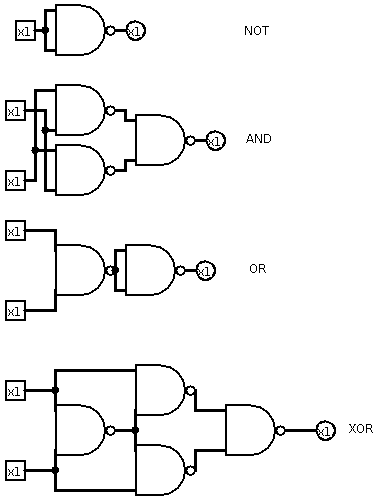
\includegraphics[scale=0.70]{circ1.png}
\end{center}
\caption{NOT-, AND-, OR- og XOR-gates af NAND-gates}
\label{fig:circ1} 
\end{figure}

\subsection{ALU, 1-bit m. overflow}
\begin{figure}[htb]
\begin{center}
\leavevmode
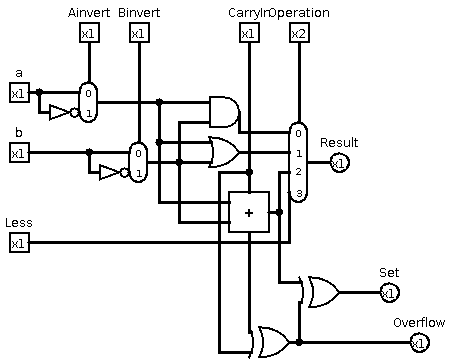
\includegraphics[scale=0.70]{alu-1bit-overflow.png}
\end{center}
\caption{1-bit ALU m. undersøgelse af overløb}
\label{fig:alu-1bit}
\end{figure}

\subsection{ALU, 1-bit u. overflow}
\begin{figure}[htb]
\begin{center}
\leavevmode
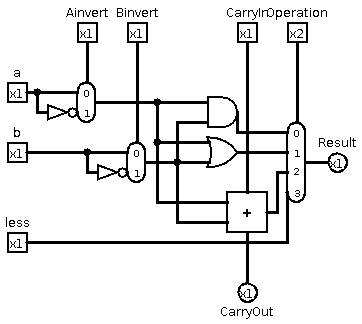
\includegraphics[scale=0.70]{alu-1bit.png}
\end{center}
\caption{1-bit ALU u. undesøgelse af overløb}
\label{fig:alu-1bit}
\end{figure}

\subsection{ALU, 4-bit}
\begin{figure}[htb]
\begin{center}
\leavevmode
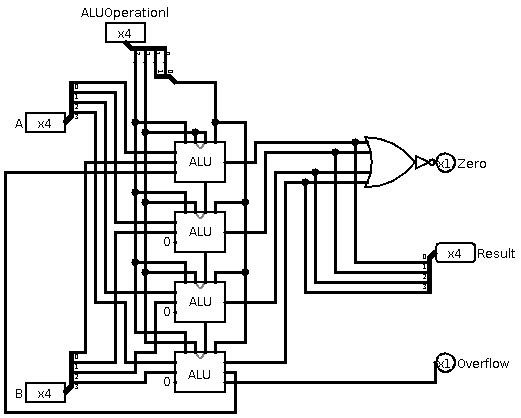
\includegraphics[scale=0.70]{circ2.png}
\end{center}
\caption{ALU, 4-bit}
\label{fig:circ2}
\end{figure}

\subsection{Adder}
\begin{figure}[htb]
\begin{center}
\leavevmode
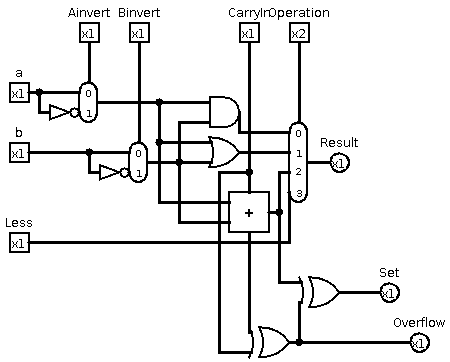
\includegraphics[scale=0.70]{adder-1bit.png}
\end{center}
\caption{1-bit adder}
\label{fig:adder}
\end{figure}

\subsection{Overløbskontrol}
\begin{figure}[htb]
\begin{center}
\leavevmode
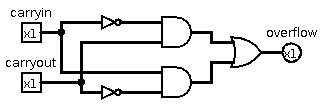
\includegraphics[scale=0.70]{overflow-detection.png}
\end{center}
\caption{Logikken til undersøgelse af overløb}
\label{fig:overflow}
\end{figure}

\subsection{Multiplexere}
\begin{figure}[htb]
\begin{center}
\leavevmode
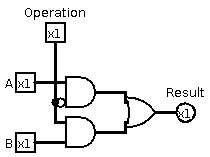
\includegraphics[scale=0.70]{mux-2bit.png}
\end{center}
\caption{MUX, 2 bit IN}
\label{fig:mux2bit} 
\end{figure}

\begin{figure}[htb]
\begin{center}
\leavevmode
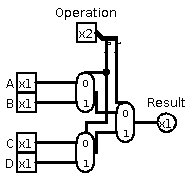
\includegraphics[scale=0.70]{mux-4bit.png}
\end{center}
\caption{MUX, 4 bit IN}
\label{fig:mux4bit} 
\end{figure}

\subsection{32-bit skifteenhed}
\begin{figure}[htb]
\begin{center}
\leavevmode
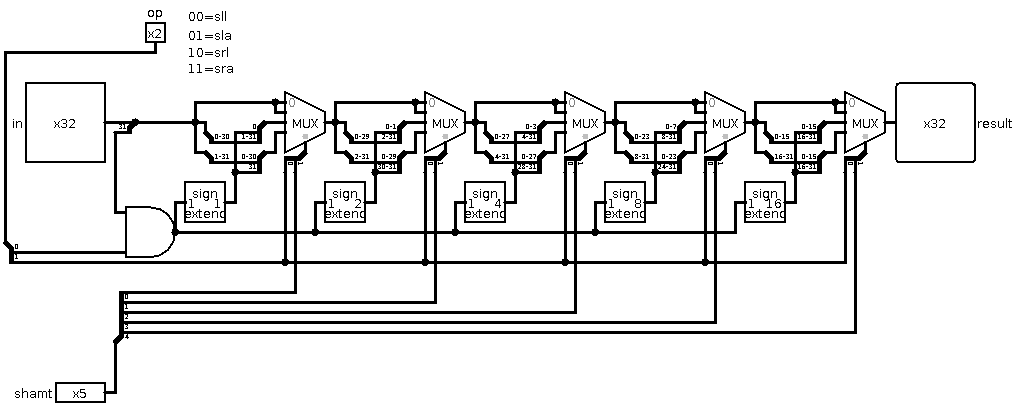
\includegraphics[scale=0.45]{circ3.png}
\end{center}
\caption{32-bit skifteenhed}
\label{fig:circ3}
\end{figure}





\end{document}
